%\chapter{det-comp}


%%%%%%%%%%%%%%%%%%%%%%%%%%%%%%%%%%%%%%%%%%%%%%
%\section{Anode Plane Assemblies}

%%%%%%%%%%%%%%%%%%%%%%%%%%%%%%%%%%%%%%%%%%%%%%
%\section{Cathode Plane Assemblies}

%%%%%%%%%%%%%%%%%%%%%%%%%%%%%%%%%%%%%%%%%%%%%%
%\section{Field Cage}

%%%%%%%%%%%%%%%%%%%%%%%%%%%%%%%%%%%%%%%%%%%%%%
\section{TPC high-voltage (HV) components}

%%%%%%%%%%%%%%%%%%%%%%%%
\subsection{Scope and requirements}

The TPC high voltage (HV) components include the HV power supply, cables,
filter circuit, feedthrough, attachment to the resistive cathode plane
arrays, the HV bus providing low-resistance connections between CPAs,
connections to the field cage, and devices for monitoring steady state
and transient conditions of current and voltage.

A schematic of the complete TPC HV circuit is shown in Figure~\ref{fig:TPCHVcircuit}.

\begin{cdrfigure}[TPC HV circuit]{TPCHVcircuit}{A schematic of the TPC high voltage circuit.}
  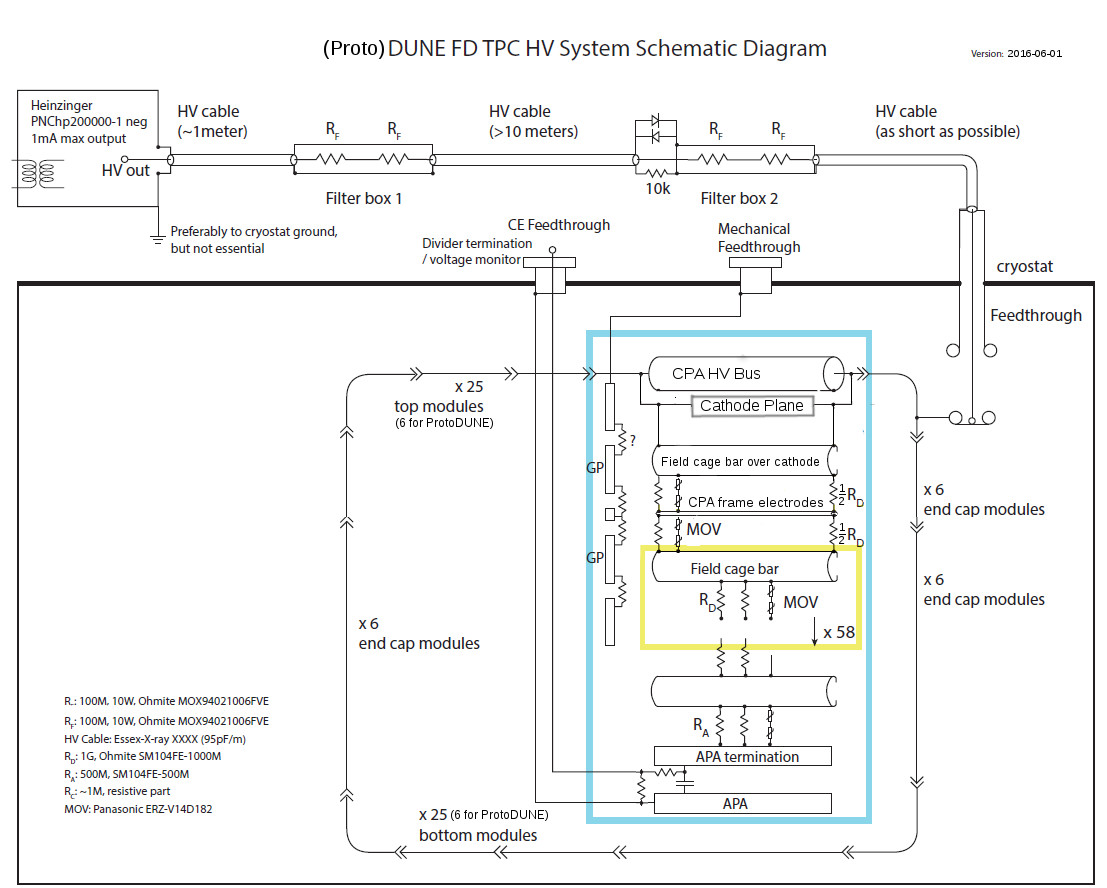
\includegraphics[width=0.95\textwidth]{VR_TPC_HV_schem-mod-1}
\end{cdrfigure}


The cathode plane will be biased at \SI{-180}{kV} to provide the
required \SI{500}{V/cm} drift field.  It will be
powered by a dedicated HV power supply through an RC filter and
feedthrough.  The power supply for the cathode plane must be able
to provide \SI{-200}{kV}.  The output voltage
ripple must not introduce more than 10\% %\fixme{(?) check ripple requirement - Gina says ok} 
of the equivalent thermal
noise from the front-end electronics. The power supply must be
programmable to shut down its output at a certain current
limit. During power on and off, including output loss (for any
reason), the voltage ramp rate at the feedthrough must be controllable
to prevent damage to the in-vessel electronics from excess charge
injection. The high-voltage feedthrough must be able to withstand \SI{-250}{kV}
at their center conductors in a \SI{1}{atm} argon gas environment when
terminated in liquid argon.

%\fixme{The above is excellent, IMHO, and should serve as a model intro.  (Anne)}
%% input from F. Pietropaolo

%%%%%%%%%%%%%%%%%%%%%%%%
\subsection{HV feedthrough design, power supply and cabling}
%In the present baseline option, 
In the design of the HV feedthrough for ProtoDUNE-SP, the procurement of the power supply and HV cables and possibly the HV filtering scheme, will take advantage of the strong synergies between the single phase and dual phase prototypes. In particular:

\begin{itemize}	
\item The Heinzinger 300-kV power supply (residual ripple less than $10^{-5}$) and the related HV cable foreseen for the DP detector are also well suited for the SP, although used at lower voltage.
\item The present DP HV feedthrough design is easily adapted to the SP without any major modification in the dimensions or in the mechanical features.
\item The filtering scheme and the monitoring system is probably more demanding on the SP detector, due to the more sensitive front-end electronics, however a common development with the DP could be advantageous, allowing to get the same HV distribution chain for both the SP and the DP protoDUNE detectors.
\item Common spare components are also planned. %envisaged.
\end{itemize}

The %present 
design of the 300-kV feedthrough is based on the very successful construction technique adopted for the ICARUS HV feedthrough, which was operated at 75~kV without interruption for more than three years without any failure. The feedthrough was also successfully operated for several days as a test after the run at 150~kV.  
%A coaxial geometry is adopted: 
The design is based on a coaxial geometry, with an inner conductor (HV) and an outer conductor (ground) insulated by UHMW PE  as shown in Figure~\ref{fig:hv-feed-through}. The outer conductor, made of a stainless-steel tube, surrounds the insulator, extending inside the cryostat up to the LAr level. %By such a 
In this geometry the electric field is %always 
confined in regions occupied by high-dielectric-strength media (UHMW PE and LAr). \fixme{Need to spell out?} The inner conductor is made of a thin-walled stainless steel tube to minimize the heat input and to avoid the creation of argon gas bubbles around the HV lower end. A contact, welded at the upper end for the
connection to the HV cable and a round-shaped elastic contact for the connection to the cathode, screwed at the lower end, completes the inner electrode. Special care has been taken in the assembly to ensure complete filling with the PE dielectric of the space between the inner and outer conductors, and to guarantee leak-tightness at ultra-high-vacuum levels.

The design of the full HV chain planned %foreseen 
for the DP detector will be finalized  after a series of tests on a prototype feedthrough and on the Heinzinger 300-kV Power Supply, which are presently ongoing at ETHZ and CERN. An alternative but similar design for the HV feedthrough is also under development at UCLA. A final decision on the design option will be based on the maximum achievable HV, reliability and stability at the design HV, and residual noise performance.
\fixme{Do we want prev pgraph?}


\begin{cdrfigure}[HV feedthrough]{hv-feed-through}{Preliminary design of the DP HV feedthrough.}
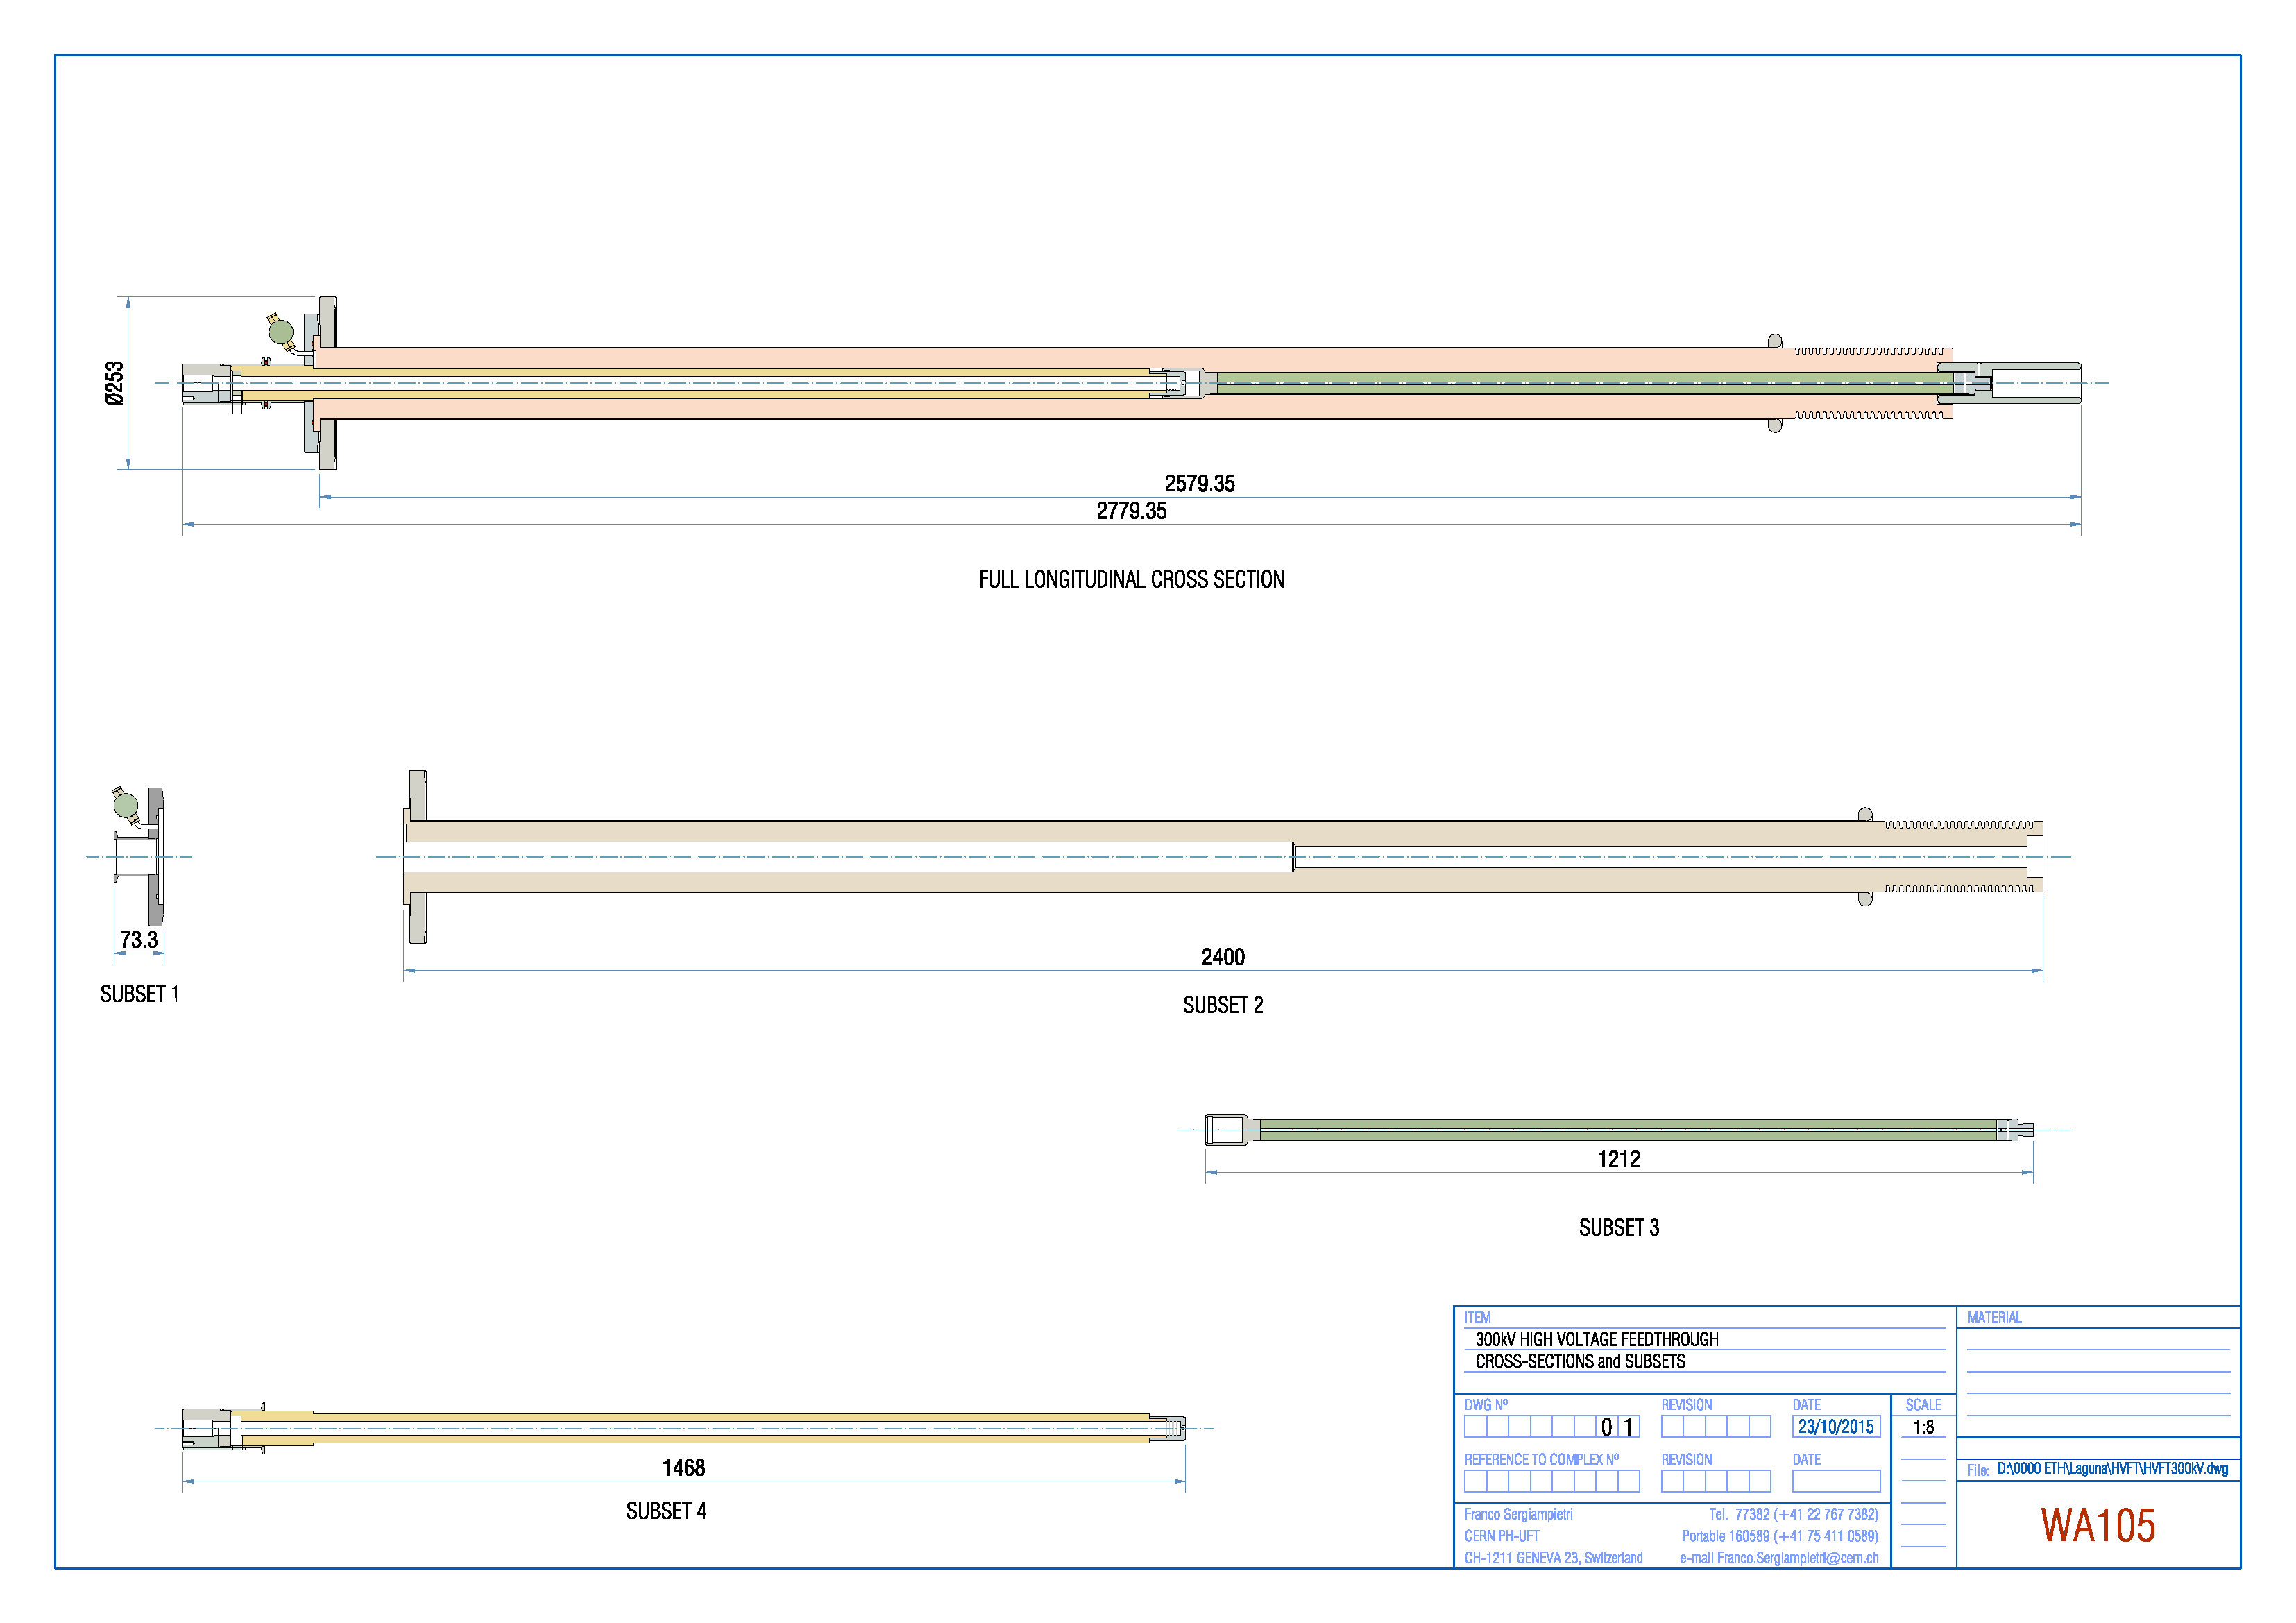
\includegraphics[width=0.95\textwidth]{tpc_HVFT300kV-1.png}
\end{cdrfigure}
\fixme{Figure~\ref{fig:hv-feed-through} could use a bit more explanation in the caption; the text of the figure is hard to read; Gina asks if we can get a photo instead}
%%




%%%%%%%%%%%%%%%%%%%%%%%%
\subsection{HV monitoring}

HV circuit monitoring devices include a toroid transformer to detect
spikes and noise in the current draw, and a monitoring point at the end
of the field cage resistor chain, which also provides a means to
control field-shaping around the edge of the
APA.

%%%%%%%%%%%%%%%%%%%%%%%%
\subsection{HV component testing}

To ensure safe and reliable operation, the HV components will be
tested at a much higher voltage than expected in routine operation
($\sim\SI{250}{kV}$) in LAr. Among these tests will be a planned
``full scale'' high voltage test at Fermilab in which all components
are subjected to the full voltage and field in liquid argon in the
35-t cryostat. \fixme{add 35-t reference here}
